\cotefile{72}
\scanpage{18}
% archive sheet number: 17

\[
\deleted{\text{b)}\quad\underbrace{\unsure{\varphi_V|2f}(a_i,a_i)}_{-2c_i}=c_i\underbrace{\langle a_i,a_i^\vee\rangle}_{-2}}
\]

\[
\text{b)}\quad\underset{\substack{\shortparallel\\2f(a_i)=2c_i}}{\varphi_V(a_i,a_i)}
=-c_i\underbrace{\langle a_i,a_i^\vee\rangle}_{-2}
\quad \underbrace{0\leq i\leq n}\quad\text{ok}
\]
\margin{$\unsure{\leq i}$}

\[
\text{c)}\quad\varphi_V(a_i,a_{i+1})=-c_i
 \underbrace{\langle a_{i+1},a_i^{\vee}\deleted{\unsure{{}_{+1}}}\rangle}_{\deleted{\unsure{\gamma_i}}\beta_i}
=-c_{i+1}\underbrace{\langle a_i\deleted{\unsure{{}_{+1}}},a_{i+1}^{\vee}\rangle}_{\deleted{\unsure{\beta_i}}\,\unsure{1}}
\quad {}^{0\leq i\leq n-1}
\]

\[
\text{i.e.}\qquad\left\{\begin{aligned}
\varphi_V(a_i,a_{i+1})&=-c_{i+1}\\
c_{i+1}&=\beta_i c_i
\end{aligned}\right.
\]

\[
c_i=(\beta_0\cdots\beta_{i-1})c_0\qquad 1\leq i\leq\unsure{i|n}
\]

donc

$f_V$ multiple de

\[
\begin{aligned}
\underbrace{f_V^0}_{\substack{\text{par la suite}\\\text{\unsure{noté|notée} }f_V}}
 \left(\sum_0^n x_i a_i\right)
 &=\sum_{i=0}^n(\beta_0\cdots\beta_{i-1})x_i^2
   +\sum_{0\leq i\leq n-1}(\beta_0\cdots\beta_i)x_i x_{i+1}\\
 &=x_0^2+\beta_0x_1^2+(\beta_0\beta_1)x_2^2+\cdots+(\beta_0\beta_1\cdots\beta_{n-1})x_n^2\\
 &\quad+\beta_0x_0x_1+\beta_0\beta_1x_1x_2+\cdots+
 (\beta_0\cdots\beta_{n-1})x_{n-1}x_n\\
 &=x_0^2+\beta_0x_1(x_0+x_1)+(\beta_0\beta_1)x_2(x_1+x_2)+\cdots\\
 &\quad+(\beta_0\cdots\beta_{n-1})x_n(x_{n-1}+x_n).
\end{aligned}
\]

% vertical bracket beside the next three handwritten lines
Donc dans $C$ il y a unique hyperquadrique $Q_C$ \deleted{\unsure{en}} invariante par \deleted{\unsure{f|\mathfrak G}} $G$, et on a donc en fait

\diagram{\begin{tikzcd}[ampersand replacement=\&]
G\arrow[r]\arrow[d,"{\times}" description]\arrow[dr,dashed,"{\times}" description] \& \operatorname{Aut}(C,Q_C)\\
\deleted{\unsure{\widetilde G|G}} \& \deleted{\operatorname{SO}(V,f_V)}\arrow[u,"{\times}" description]
\end{tikzcd}}
% The two lower objects and the three connecting arrows are crossed out together.
\scanpage{19}
% archive sheet number: 18

Ceci nous amène \unsure{à|:} introduire

\[
\boxed{C_0'''}=\text{Cat. des }\deleted{\text{triples}}\inserted{\text{quadruples}}\ 
(C,Q_C,\varphi_G^{C\deleted{\unsure{G}}},h_0),
\]

\margin{\uline{NB} $n\geq 2$}
$C$ fibré projectif de rg $n$, $Q_C$ hyperquadrique dans $C$, $\varphi_G^C:G\unsure{\relbar|\longrightarrow}\operatorname{Aut}(C,Q_C)$, $h_0$ section de $C$, satisfaisant les conditions

a) les $\tau_i^C\overset{\mathrm{dfn}}=\varphi_G^C(\underline{\tau}_i)$ sont des ps. réfl., strictes si $1\leq i\leq n$, et associée à $h_0$ si $i=0$ (peut être triviale si $i=0$)
\[
\Rightarrow\ \begin{aligned}
h_i&\quad(1\leq i\leq n)\\
H_i&\quad(1\leq i\leq n)
\end{aligned}
\]
\margin{\uline{NB} $\tau_0^C$ est \unsure{str. ortho.|strict. ortho.} ssi \unsure{s'est|c'est} une réflexion stricte, i.e. ssi \deleted{$\beta_0\ne 0$} \inserted{en chaque $\mathrm{p}^\mathrm{t}$} $\forall s,\ \beta_0(s)\ne 0$ ou $\unsure{k|K}(s)$ de car. $\ne 2$}

b) Les $h_i$ lin. indép. en chaque fibre

c) $h_i\notin H_{i+1}$ en $\forall$ fibre \quad $(0\leq i\leq n-1)$

\deleted{\uline{NB} Si $Q_C$ est lisse, \inserted{et \deleted{\unsure{les}} $\tau_0$ \uline{stricte} ($\ne\mathrm{id}$ en chaque fibre)} alors \unsure{on a} \unsure{équivaut|équivat|équivalent} : $\forall i$, $H_i$ est l'orth. de \unsure{$h_i$}}

\uline{NB} Supposons les $\tau_i$ stricts orthogonaux \inserted{dans $C$ \deleted{\illegible{1}}} i.e. les $\beta_i$ inv. (C'est le cas si $Q_C$ est lisse \ldots) Alors la condition c) équivaut à

\[
\begin{aligned}
\text{c$'$)}\ (\tau_i\tau_{i+1})^2&=\mathrm{id}\quad\text{sur chaque fibre,}\\
\text{i.e.}\quad \tau_i&\ \text{ne commute pas à }\tau_{i+1}\text{ en chq fibre}
\end{aligned}
\ \Big|\ 0\leq i\leq n-1
\]

La condition b) s'énonce ainsi

b$'$) En $\forall\, s\in S$, la repr. \inserted{de $G$} induite sur $C_s$ est irréductible [suffisance claire, pour la nécessité il faut travailler un peu \ldots]
\margin{?}
\scanpage{20}
% archive sheet number: 19

A) Cas $n$ pair $\geq 2$, donc $C$ de rang $n$ pair aussi donc $V$ de rang impair, donc
\[
\operatorname O(f_V)\supset\operatorname{SO}(f_V)\times\mu_2,\quad\text{et}
\]
\diagram{\begin{tikzcd}[ampersand replacement=\&]
\operatorname{SO}^{\unsure{\circ}}(f_V)\arrow[r,hook]\&\operatorname{Aut}(C,Q_C)
\end{tikzcd}}

En fait, l'hom
\diagram{\begin{tikzcd}[ampersand replacement=\&]
G\arrow[r,"{\varphi_G^C}"]\&\operatorname{Aut}(C,Q_C)
\end{tikzcd}}

se factorise à travers $\operatorname{SO}(f_V)$
\diagram{\begin{tikzcd}[ampersand replacement=\&]
G\arrow[r,"{\psi_G^V}"]\&\operatorname{SO}(f_V)
\end{tikzcd}}

On notera que
\[
\psi_{\unsure{G}}^V(\underline{\tau}_i)=-\varphi_G^V(\underline{\tau}_i)=-\tau_i^V
\]

\uline{Ex} \uline{$n=2$,} \deleted{alors \unsure{$Q$}} Supposons $f_V$ lisse\deleted{\unsure{en|lisse}} i.e. $Y=Q_C$ un fibré en droites projectives i.e.
\[
\underset{\substack{\shortparallel\\\alpha_0+2}}{\beta_0},\
\underset{\substack{\shortparallel\\\alpha_1+2}}{\beta_1}
\ \text{et}\ \beta_0+\beta_1-4=\alpha_0+\alpha_1\ \text{inv.},\quad\text{alors}
\]
\[
\operatorname{SO}(f_V)\xrightarrow{\sim}\operatorname{Aut}(Q_C),
\]
donc la donnée de $C$ et $\varphi_G^C$ ou $\psi_G^V$ équivaut à \deleted{celle} du fibré en droites projectives $Y$ $(=Q_C)$, et de l'opération de $G$ dessus via $\tau_0^Y,\tau_1^Y,\tau_2^Y$. Traduisons les conditions explicitées plus haut sur $\unsure{\psi_G^C|\varphi_G^C}$ en termes de $\varphi_G^Y$ (\uline{NB} ici $\beta_0$ inv. donc $\tau_0$ \unsure{réflexion|psflexion} stricte, donc $h_0$ s'en déduit \unsure{de|du} l'\unsure{enveloppe|un} \unsure{$2$-projective|$2$-projectiv.|$2$-rejet} $C$ de $Y$)
\scanpage{21}
% archive sheet number: 20

1) $\forall\,0\leq i\leq2$, $\tau_i^C$ est $\ne 1$ en chaque fibre $\left(\Rightarrow
\begin{array}{ccc}h_0,&h_1,&h_2\\ H_0,&H_1,&H_2\\\multicolumn{3}{c}{\text{dans } C}\end{array}\right]$

2) $h_0\ h_1\ h_2$ lin. indép. en chaque fibre

\deleted{(à \unsure{expliciter} \inserted{\unsure{plus intrinsèque}} en termes de $\unsure{\varphi_G^Y}$)}

$\Longleftrightarrow$ \deleted{$\forall$} $\forall$ fibre \deleted{\unsure{générique}} $Y_{\bar s}$, il \uline{n'existe pas} de diviseur $\Delta$ de $Y_{\bar s}$ de degré $2$, invariant par $\varphi_G^Y$, i.e. pas de restriction à une structure soit de droite affine, soit de \deleted{droite affine} torseur sous $\mathrm G_m$ \ldots\ (avec $G$ agissant sur $\mathrm G_m$ \ldots)

% slanted
\margin{C'est sans doute ce qui exclut le cas ``\unsure{diédral|dièdral}''}

3) $\tau_0^C\tau_1^C\overset{\mathrm{dfn}}=\rho_f$ et $\tau_1^C\tau_2^C\overset{\mathrm{dfn}}=\rho_s$ sont tels que
\[
\rho_f^2\ne\mathrm{id}_{\unsure{Y|C}},\quad \rho_s^2\ne\mathrm{id}_Y\quad\text{sur chaque fibre.}
\]

(cela exprime la non commutation de $\tau_0,\tau_1$, et de $\tau_1,\tau_2$, sur chaque fibre
\scanpage{23}
% archive sheet number: 22

\unsure{6|§|(} Automorphismes de $X$ $(=\mathrm P(\unsure{E|\mathcal E}))$ induisant l'identité sur $C$.

Ils correspondent aux pseudo-reflexions de $E$ qui sont l'identité sur $V$, donc de la forme
\[
u=\mathrm{id}+\pi\otimes a\tag*{(1)}
\]
$a$ section de $E$. Si on écrit que $u$ commute aux $\tau_i$, cela s'écrit $\langle a,a'_i\rangle=0$ $(0\leq i\leq n)$ i.e. $a$ de la forme $\lambda\widetilde o$
\[
u=\mathrm{id}+\pi\otimes\lambda\widetilde o\tag*{(2)}
\]

Écrivons que $u$ est orthogonale, i.e.
\[
\underbrace{f(\deleted{\unsure{a|\lambda}}\lambda\widetilde o)}_{-\lambda^2\sigma'\rho'}\pi+
\underbrace{\psi(\lambda\widetilde o)}_{-\lambda\sigma\pi}=0
\]

ou encore
\[
\lambda(\lambda\sigma'\rho'+\sigma)=0\tag*{(3)}
\]
ce qui suivant la parité de $n$ s'écrit
\[
\left\{\begin{aligned}
 &n\text{ pair }(\rho=2\rho',\underline{\sigma=\sigma'})&
 \lambda\sigma'(\lambda\rho'+1)&=0\\
 &n\text{ impair }(\underline{\rho=\rho'},\sigma=2\sigma')&
 \lambda\sigma'(\lambda\rho^{\deleted{\unsure{\prime}}}+2)&=0
\end{aligned}\right.\tag*{(4)}
\]

D'autre part, la \deleted{fait} \inserted{condition} que $u$ soit une \uline{reflexion} s'écrit $\langle\lambda\widetilde o,\pi\rangle=-2$ i.e.
\[
\lambda\rho=-2\tag*{(5)}
\]

\deleted{\unsure{$n$ pair}} S

\uline{Proposition} 1) Si $\sigma'=0$, \unsure{alors|tous|toutes} les \deleted{\unsure{auto|autres}} \deleted{\unsure{qui}} pseudo-reflexions \deleted{telles que} \inserted{commutant à $G$ et} fixes sur $V$ sont orth.

2) Si $\sigma'$ inv, \deleted{une}\inserted{la} ps. reflexion $u=\mathrm{id}+\lambda\pi\otimes\widetilde o$
\scanpage{24}
% archive sheet number: 23

est orth ssi elle satisfait à $\lambda\rho'+1=0$ (cas $n$ pair) resp $\underbrace{\lambda\rho+2}_{=\lambda\rho'+2}=0$ (cas $n$ impair).

Donc

a) Si $n$ pair, $\exists$ une telle $u$ \inserted{$\ne\mathrm{id}$ sur tte fibre} ssi $\rho'$ inv, et on a alors unicité :
\[
u=\mathrm{id}-\pi\otimes o'\qquad o'=\frac1{\rho'}\widetilde o\tag*{(6)}
\]
i.e. $u$ est l'\uline{antipodisme}

b) Si $n$ impair, \inserted{$2$ inv}, \deleted{$\exists$ une telle $u$ ssi} \inserted{pour qu'il} \deleted{$\rho$ est \unsure{inv|inv.}, $\exists!u$} \deleted{ou bien $\rho$.} existe une telle $u$, il \deleted{faut} \inserted{f. et} suffit que $\rho' (=\rho^{\deleted{\unsure{\prime|*}}})$ soit inv, \deleted{et $2$ inv.} \deleted{cette condition est néc.} \deleted{et alors cette condition est} \deleted{\unsure{néc. si} $2$ inv.} On a alors unicité,

% margin note written sideways
\margin{dans ce cas, $u$ \unsure{invarie|inverse|invariant} donc automatiquement la \unsure{réal.|virt.} \unsure{géom|géom.} envisagée de $\Pi$}

$\lambda=-\dfrac2\rho=-\dfrac2{\rho'}$ i.e.
\[
u=\mathrm{id}-\pi\otimes\frac{2\widetilde o}{\rho'}\tag*{(7)}
\]
et $u$ est encore l'\uline{antipodisme}.

c) Si \inserted{$n$ impair,} $S$ de car. $2$, \deleted{alors $\exists$ un} \deleted{ssi $\rho$ est} \inserted{pour qu'il existe,} une telle $u$, il \deleted{\unsure{faut}} faut que $\rho(=\rho')$ \deleted{soit} \unsure{nilpotent}, et suffit que \deleted{$\rho=\rho'$ soit \unsure{nul}} \deleted{\unsure{soit inv.}} Dans ce dernier cas, \unsure{tte} pseudo reflexion qui est identité sur $V$ et commute à $G$ est orthogonale,

% slanted
\margin{(La condition néc et suff. est donc $\rho'=0$, \deleted{\unsure{dans}} \inserted{\unsure{le cas|les cas}} \unsure{lorsque} $S$ réduit)}

\deleted{en particulier}

En particulier

\uline{Corollaire} Supposons $\sigma'\rho'$ inv. i.e. $f(\widetilde o)$ inv. i.e. $c\ \deleted{\unsure{\notin}}\in\Gamma(X\setminus Q_X)$, \deleted{en ttes fibres} i.e. $o\notin Q_X$ en tte fibre, \inserted{\uline{et} $2$ inv. sur $S$ si $n$ impair.} Alors, et alors seulement, \deleted{lors que $G$} $\exists$ unique $G$-automorphisme $\ne\mathrm{id}$ sur chaque fibre, induisant l'identité sur $C$. et invariant $Q_C$. Ce dernier est l'antipodisme.
\scanpage{25}
% archive sheet number: 24

\uline{NB} L'antipodisme peut être défini \inserted{intrinsèquement} indépendamment de tte condition de caractéristique, et quelle que soit la parité de $n$, dès que $\rho'$ est inversible, \inserted{grâce à (6), (7)}. \deleted{(Mais pour $n$ impair et} \inserted{Pour que $u$ soit} l'identité, il faut s. que $n$ impair et $S$ de car. $2$. Donc pour qu'il soit $\ne\mathrm{id}$ en chaque fibre, il f. et s. que $n$ pair ou $2$ inv. sur $S$.

\begin{center}\rule{1.1cm}{0.4pt}\\[-.6ex]\rule{.9cm}{0.4pt}\end{center}

Considérons $G\xrightarrow{\varphi_G}\operatorname{Aut}(X)$ satisfaisant les conditions habituelles (mais on ne donne pas pour l'\unsure{instt|instant} de réal$^{\mathrm n}$ géom. corr., i.e. pas de $s_0$\ldots). Donc on a $C\subset X$ permettant de construire (
\diagram{\begin{tikzcd}[ampersand replacement=\&]
0\arrow[r]\&V\arrow[r]\&E\arrow[r]\&\underline{\mathcal O}_S\arrow[r]\&0
\end{tikzcd}}
\margin{$X=\check{\mathbb P}(\unsure{E|\mathcal E})$}

et on a $L_i\subset V,\ L'_i\subset\check V_{\deleted{\unsure{S}}}$ $(0\leq i\leq n)$, \deleted{$L_i\subset\check V$} tels que $V=\bigoplus L_i$, \deleted{$\unsure{V'|\check V}=\bigoplus L'_i$}, $L_i\otimes L'_{i+1}\overset{\sim}{\longrightarrow}\underline{\mathcal O}_S$ pour $0\leq i\leq n-1$. \deleted{En \unsure{f|p} Considérons la} \inserted{Ainsi,} $G$ opère sur $V$ \deleted{\unsure{via}} de façon compatible avec son op sur $C\simeq\check{\mathrm P}(V)$. On a en \unsure{loc$^{\mathrm{ment}}$|laissant|outre} la donnée de $s_0$ (satisfaisant aux conditions habi%
\scanpage{26}%
% archive sheet number: 25
tuelles) permet de définir des sections $a_i,a'_i$ de $V,\check V$ -- en fait, $a'_0$ est une section de $L'_0$ définie en termes de \deleted{$D_{s_0}$} la \deleted{droite} \inserted{section} $s_0$ de $\unsure{E|\mathcal E}$ \deleted{$\Delta_{\unsure{s|\xi}}\subset E$ \unsure{engendrée par} $s_0$ et} \inserted{(au dessus de $1$,} définissant un \unsure{splittage|splitting} de $E$ en $E\simeq V\oplus\underline{\mathcal O}_S$ \ldots) par $\langle s_0,a'_0\rangle=1$, ce qui permet ensuite de définir de proche en proche les bases $a_0,a'_1,a_{\unsure{2|1}},\ldots,a'_n,a_n$ de $L_0,L'_1,L_1,\ldots$ par les conditions
\[
\tau_i^E=\mathrm{id}+a'_i\otimes a_i,\quad
\langle a_i,a'_{i+1}\rangle=1\qquad 0\leq i\leq n
\]
(\uline{NB} il y a lieu de poser $a_{-1}=s_0$\unsure{.})

Inversement, donnons nous une base $a'_0$ de $L'_0$. \deleted{Considérons \unsure{ce que veut|indique voir}} le plan
\[
F=\bigcap_{1\leq i\leq n}\mathcal H_i\qquad
\text{orthogonal aux}\quad L'_i\quad 1\leq i\leq n,
\]
\deleted{dans celui-ci l'équation} on a \deleted{$\mathcal H_0\cap F$} $F\not\subset\mathcal H_0$ en tte fibre i.e. $F\cap\mathcal H_0$ est une droite (la droite $\Delta_{\unsure{o|0|c}}$ \deleted{\unsure{engendrée}} $\subset E$ correspondant à $o$), et l'équation \deleted{$\unsure{\xi}$} $\langle s,a'_0\rangle=1$ définit dans $F$ une \deleted{\unsure{translat.}} \inserted{droite affine} \deleted{\unsure{lin.}} translatée de $\Delta$, soit $\Delta'$ (dépendant du choix de $a'_0$ -- \deleted{\unsure{il y a une bijection}} (\uline{NB} : $L'_0\simeq F/\Delta$)

Considérons $F\xrightarrow{\pi|F}\underline{\mathcal O}_S$
\scanpage{27}
% archive sheet number: 26

(4p)

forme hermitienne invariante pour un hyperpolyèdre régulier
\scanpage{28}
% archive sheet number: 27

\[
\varphi(a_j,a_{\unsure{l|k|i}})=0\quad -1\leq j<l\leq n,\ l\ne j+1,\quad
\varphi(a_{-1},a_{-1})=f(a_{-1})=0
\]

\[
\begin{aligned}
0\leq i\leq n\qquad &c_i=f(a_i)=\varphi(a_i,a_i)\\
0\leq i\leq n\qquad &\lambda_i-1=\langle a_i,a'_i\rangle\\
0\leq i\leq n-1\qquad &\beta_i=\langle a_{i+1},a'_i\rangle\\
-1\leq i\leq n-1\qquad &\langle a_i,a'_{i+1}\rangle=1
\end{aligned}
\]

\[
\boxed{\begin{aligned}
&\left\{c_i\langle a_j,a'_i\rangle\deleted{\unsure{+|=|-}}\inserted{=}\overbrace{(\lambda_i-1)}^{\mu_i}\varphi(a_j,a_i)=0\right.\\
&0\leq i,\deleted{\unsure{j}}{}\leq n\qquad\lambda_i\overline{\lambda_i}=1\\
&-1\leq j\leq n
\end{aligned}}
\]
\[
\left[f(a)a'=\underbrace{\langle a,a'\rangle}_{\mu=\lambda-1}\psi(a)\right]
\]
\[
\tau x=x+\left(\frac{\mu}{f(a)}\varphi(x,a)\right)a,\qquad \lambda\bar\lambda=1
\]

\[
d_i=\frac{c_i}{\lambda_i-1}=\varphi(a_{i-1},a_i)\quad
0\leq i\leq n\qquad\text{i.e.}\quad c_i=(\lambda_i-1)d_i=\mu_i d_i
\]
\[
d_{i+1}=\overline{\beta_i}\,\overline{d_i}\qquad\text{donc}
\]
\[
\begin{aligned}
d_1&=\overline{\beta_0}\,\overline{d_0}\\
d_2&=\overline{\beta_1}\,\beta_0 d_0\\
d_3&=\overline{\beta_2}\,\beta_1\overline{\beta_0}d_0\\
&\cdots\\
d_{\deleted{\unsure{2i-1}}2i}&=\overline{\beta_{2i-1}}\beta_{2i-2}\overline{\beta_{2i-3}}\cdots\beta_0d_0\\
d_{2i+1}&=\overline{\beta_{2i}}\beta_{2i-1}\overline{\beta_{2i-2}}\cdots\overline{\beta_0}\,\overline{d_0}\\
&\cdots\\
d_{\unsure{n|n+1}}&=\overline{\beta_{n-1}}\beta_{n-2}\overline{\beta_{n-3}}\cdots
\left\}\begin{array}{ll}\beta_0d_0&\text{si }n\text{ pair}\\\overline{\beta_0}d_0&\text{si }n\text{ impair}\end{array}\right.
\end{aligned}
\]
\[
d_0=\frac{c_0}{\lambda_0-1}=\frac{c_0}{\mu_0}\ \Big|\ \underline{c_0\in k_0}
\qquad \text{OPS }c_0=1,\ \text{donc }d_0=\frac{1}{\mu_0}
\]

\[
\begin{aligned}
f(a_{-1})&=0\\
f(a_0)&=1\\
f(a_1)&=\frac{\mu_1\deleted{\unsure{1}}}{\overline{\mu_0}\deleted{\unsure{1}}}\overline{\beta_0}\\
f(a_2)&=\frac{\mu_2\deleted{\unsure{-1}}}{\mu_0^{\deleted{\unsure{\overline{\phantom{a}}}}}\deleted{\unsure{-1}}}\overline{\beta_1}\beta_0\\
f(a_3)&=\frac{\mu_3}{\overline{\mu_0}}\overline{\beta_2}\beta_1\overline{\beta_0}\\
&\cdots
\end{aligned}
\]

Supposons les $\beta_i\in k_0$, il reste les conditions
\[
\begin{aligned}
\mu_i/\mu_0^{\deleted{\unsure{\bar{\phantom{a}}}}}&\in k_0\quad\text{si }\unsure{0|i}\text{ pair}\\
\mu_{\unsure{i|1}}/\overline{\mu_0}&\in k_0\quad\text{si }i\text{ impair}
\end{aligned}
\]

\[
\begin{aligned}
\deleted{\unsure{\text{Si }\lambda}}\quad\lambda_i-1&=\rho_i(\lambda_0-1)
\quad \inserted{\text{($\rho_i\in k_0$)}}\quad i\text{ pair}\\
\lambda_i&=\rho_i(\lambda_0-1)+1\qquad\unsure{\rho}\\
\deleted{\unsure{\lambda_i\overline{\lambda_i}}}&=(\lambda_0-1)\unsure{\bar\rho_i|\bar\varphi_i|\varrho_i|q_i}
\end{aligned}
\]

\deleted{\unsure{Or}} \deleted{\unsure{Supp.}}

\[
(\lambda_1-1)=\deleted{\unsure{\rho}}c(\overline{\lambda_0}-1)
\]

\figure{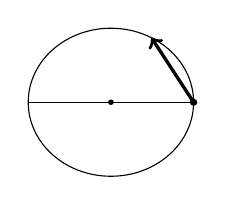
\begin{tikzpicture}[x=1.05cm,y=1cm]
\draw (0,0) ellipse (1 and .94);
\draw (-1,0) -- (1,0);
\fill (0,0) circle (.035);
\fill (1,0) circle (.045);
\draw[very thick,->] (1,0) -- (.49,.82);
\end{tikzpicture}}
\scanpage{29}
% archive sheet number: 28

\[
\begin{aligned}
\tau_0\tau_1&=\begin{pmatrix}\lambda_0+\beta&\beta\lambda_1\\1&\lambda_1\end{pmatrix}
&\operatorname{Tr}\tau_0\tau_1&=\lambda_0+\lambda_1+\beta\\
&&\ \shortparallel&\\
\tau_1\tau_0&=\begin{pmatrix}\lambda_0&\beta\\\lambda_0&\lambda_1+\beta\end{pmatrix}
&\operatorname{Tr}\tau_1\tau_0&\qquad\det\tau_0\tau_1=\lambda_0\lambda_1
\end{aligned}
\]

\deleted{$\unsure{\varphi^2-2|\text{Ex. }2}$}
\[
\begin{aligned}
A(\tau_0\tau_1)
&=\frac{(\lambda_0+\lambda_1+\beta)^2}{(\lambda_0\lambda_1)}-2
=\frac{\lambda_0}{\lambda_1}+\frac{\lambda_1}{\lambda_0}+
\frac{\beta^2}{\lambda_0\lambda_1}+2\beta\left(\frac1{\lambda_0}+\frac1{\lambda_1}\right)\\
\unsure{z}&=\underbrace{\lambda_0\overline{\lambda_1}+\lambda_1\overline{\lambda_0}}_{\substack{\unsure{\rotatebox{90}{$\in$}|\uparrow}\\\mathbb R}}
+\beta^2\cdot\overline{\lambda_0}\,\overline{\lambda_1}
+2\beta(\overline{\lambda_0}+\overline{\lambda_1})\\
&=\left\{\begin{array}{l}-2\\-1\\0\\\alpha,\alpha'\end{array}\right.
\end{aligned}
\]

\[
\begin{aligned}
(\tau_0\tau_1)^2&\ne 1\\
\tau_0\tau_1\tau_0\tau_1&=\\
(\lambda_0\lambda_1)^2&=1\qquad\unsure{)}
\end{aligned}
\]

\[
\beta=c\frac{(\lambda_0-1)\deleted{\unsure{\lambda_1}}}{(\overline{\lambda_1}-1)}
\]

\[
\underline{\lambda_0+\lambda_1+\beta}
\]
\diagram{$\begin{array}{c@{}ccc}
 &2&2&2\\[-.2ex]
\unsure{\in|(}&3&3&3\\
 &4&4&4\\
 &5&5&5
\end{array}$}

\[
\begin{aligned}
&(\overline{\lambda_1}-1)^2(\lambda_0\overline{\lambda_1}+\lambda_1\overline{\lambda_0})
+c^2(\lambda_0-1)^2\overline{\lambda_0}\,\overline{\lambda_1}\\
&\deleted{+2(\lambda_0-1)(\overline{\lambda_1}\unsure{1|-1})}\\
&\lambda_0^2+\lambda_1^2+\beta^2+2\beta(\lambda_0+\lambda_1)\\
&(\lambda_0^2+\lambda_1^2)(2-k_1)^2+c^2(\unsure{\lambda_0-\lambda_0|\lambda_0-1|\lambda_0-\overline{\lambda_0}})^2(\lambda_1-1)^2\\
&\qquad+2c(2-k_1)(\lambda_0-1)(\lambda_1-1)(\lambda_0+\lambda_1)\\
&\hspace{15em}=k
\end{aligned}
\]

\[
\frac c{2-k_1}=x
\]

\[
\begin{array}{ccc}
\tau_0&\tau_1&\tau_\infty\\p&q&r
\end{array}
\]

\tikz[baseline=(p.base)]{\node[inner sep=2pt] (p) {\textcircled{1} un des trois $p,q,r=2$};\draw (p.north east) .. controls ([yshift=1.2ex]p.north west) and ([xshift=-1em]p.west) .. (p.south west) .. controls (p.south) .. (p.south east);}

déjà traité,

$p,q,r\geq3$
\[
x^2+\left(2\deleted{\unsure{(2-k_1)}}\,
\overbrace{\frac{\lambda_0+\lambda_1}{(\lambda_0-1)(\lambda_1-1)}}\right)x+
\left[\deleted{\unsure{(2-k_1)^2}}\frac{\lambda_0^2+\lambda_1^2}{(\lambda_0-1)^2(\lambda_1-1)^2}-k\right]=0
\]

solutions \uuline{réelles}\qquad $k=-2\deleted{\unsure{4}},-1,0,1,\alpha,\alpha'$
\scanpage{30}
% archive sheet number: 29

% Long diagonal strokes cancel the upper calculation.
\[
\begin{aligned}
&\deleted{A(\tau_0\tau_1)=\frac1{\lambda_0\lambda_1}
\left(\beta^2+2(\lambda_0+\lambda_1)\beta+(\lambda_0^2+\lambda_1^2)\right)}\\
&\deleted{=\underbrace{\frac{(\lambda_0-1)^2(\lambda_1-1)^2}{\lambda_0\lambda_1}}_{16\sin^2\frac{\theta_0}{2}\sin^2\frac{\theta_1}{2}}
\left({\unsure{\zeta|\gamma|\beta}}^2+2\underbrace{\frac{(\lambda_0+\lambda_1)}{(\lambda_0-1)(\lambda_1-1)}}_{-\frac{\cos\frac{\theta_1-\theta_0}{2}}{\sin^{\deleted{\unsure{2}}}\frac{\theta_0}{2}\sin\frac{\theta_1}{2}}}\zeta
+\underbrace{\frac{\lambda_0^2+\lambda_1^2}{(\lambda_0-1)^2(\lambda_1-1)^2}}_{\frac18\frac{\cos(\theta_1-\theta_0)}{\sin^2\frac{\theta_0}{2}\sin^2\frac{\theta_1}{2}}}\right)=k}
\end{aligned}
\]

\[
\begin{aligned}
&\deleted{(\lambda_i-1)^2\quad\arg.\ \theta_i+\pi}\\
&\deleted{(\lambda_0-1)^2(\lambda_1-1)^2\quad\arg\ \underline{\theta_0+\theta_1}+2\pi}\\
&\deleted{\lambda_0\lambda_1\quad\arg\ \theta_0+\theta_1}\\
&\deleted{\underline{16\sin^2\frac{\theta_0}{\unsure{1|2}}\sin^2\frac{\theta_1}{2}}}
\end{aligned}
\]

\[
\deleted{\underline{k=-2+\psi\qquad k+2=\psi}}
\]
\[
\begin{aligned}
&\deleted{\beta_i=\zeta_i(\lambda_i-1)(\lambda_{i+1}-1)\qquad \lambda_i-1=\mu_i\ \text{\unsure{unités|unité}}}\\
&\deleted{\phantom{\beta_i}=\zeta_i\mu_i\mu_{i+1}}\\
&\deleted{\unsure{d_i=\frac{c_i}{(\lambda_i-1)}=\zeta_i(\lambda_i-1)}}
\end{aligned}
\]
\[
\deleted{d_{i+1}=\zeta_i(\overline{\lambda_i}-1)(\overline{\lambda_{i+1}}-1)d_i}
\]
\[
d_{i+1}=\overline{\mu_i}\,\overline{\mu_{i+1}}\,\zeta_i
\]
\deleted{\unsure{donc}}

\[
\begin{aligned}
c_i&=f(a_i)=\varphi(a_i,a_i)\qquad 0\leq i\leq n\\
(c_{-1}&=f(a_{-1})=\varphi(a_{-1},a_{-1})=0)\\
d_i&=\frac{c_i}{\deleted{\unsure{\lambda_i}}\mu_i}=\varphi(a_{i-1},a_i)\\
\mu_i&=\lambda_i-1
\end{aligned}
\]

\[
\begin{aligned}
1)\quad &\varphi(a_i,a_j)=0\quad -1\leq i<j\leq n,\quad i,j\text{ non cons.}\\
2)\quad &\varphi(a_{i-1},a_i)=\frac{c_i}{\mu_i}\deleted{\unsure{=\lambda_i}}\overset{\mathrm{dfn}}=d_i\qquad0\leq\unsure{i|0}\leq n\\
&\deleted{3}
\end{aligned}
\]

\deleted{donc $c_i=\unsure{\mu_i|\overline{\beta_i}\mu_i}d_i$}

posons
\[
\boxed{\begin{aligned}
\beta_{\unsure{i|r}}&=\zeta_i\mu_i\mu_{i+1}\\
\text{i.e.}\quad \zeta_i&=\frac{\beta_i}{\mu_i\mu_{i+1}}
\qquad 0\leq i\leq\unsure{n|n-1},
\end{aligned}}
\]
\[
\begin{aligned}
3)\quad d_{i+1}&=\overline{\beta_i}\,\overline{d_i}\qquad 0\leq i\leq n-1\\
\text{i.e.}\quad d_{i+1}&=\overline{\zeta_i}\,\overline{\mu_i}\,\overline{\mu_{i+1}}\,\overline{d_i}\\
\text{\deleted{donc}}\quad\deleted{\unsure{d_{i+1}}}\ \frac{c_{i+1}}{\mu_{i+1}}&=
\overline{\zeta_i}\deleted{\overline{\mu_i}}\,\overline{\mu_{i+1}}\,\frac{\overline{c_i}}{\deleted{\overline{\mu_i}}}
\end{aligned}
\]
\[
\text{i.e.}\quad\deleted{c_{i+1}=N(\mu_{i+1})\overline{c_i}\overline{\zeta_i}}\qquad
 c_{i+1}=N(\mu_{i+1})\overline{\zeta_i}c_i\quad\searrow\zeta_i\in k_0
\]

donc
\[
\begin{aligned}
&\deleted{d_1=\overline{\zeta_0}\,\overline{\mu_0}\,\overline{\mu_1}}\\
&\deleted{d_2=\overline{\zeta_1}\,\overline{\mu_1}\,\overline{\mu_2}\zeta_0\mu_0\mu_1
=(\overline{\zeta_1}\zeta_0)\overline{\mu_2}N(\mu_1)\mu_0}\\
&\deleted{d_3=\overline{\zeta_2}\,\overline{\mu_2}\,\overline{\mu_3}\overline{[\,\phantom{x}\,]}
=(\overline{\zeta_2}\zeta_1\overline{\zeta_0})\overline{\mu_3}N(\mu_2)N(\mu_1)\overline{\mu_0}}
\end{aligned}
\]

\deleted{\unsure{NB}}
\[
\left\{\begin{aligned}
c_0&=1\\
c_1&=N(\mu_1)\zeta_0\\
c_2&=N(\mu_1\mu_2)\zeta_0\zeta_1\\
c_3&=N(\mu_1\mu_2\mu_3)\zeta_0\zeta_1\zeta_2\\
&\hbox to 2em{\hrulefill}\\
c_n&=N(\mu_1\cdots\mu_n)\zeta_0\cdots\zeta_{n-1}
\end{aligned}\right.
\]
\[
\begin{aligned}
\varphi(a_{i\unsure{+|-}1},a_i)&=\frac{c_i}{\mu_i}=N(\mu_0\cdots\mu_{i-1})\overline{\mu_i}(\zeta_0\cdots\zeta_{i-1})\\
\varphi(a_i,a_{i-1})&=N(\mu_0\cdots\mu_{i-1})\mu_i(\zeta_0\cdots\zeta_{i-1})
\end{aligned}
\]
\scanpage{31}
% archive sheet number: 30
% One long diagonal cancellation runs from the first calculation to the last.

\[
\begin{aligned}
&\deleted{f(a_0)=1}\\
&\deleted{f(a_1)=\frac{\mu_1}{\overline{\mu_0}}\overline{\beta_0}=c\in k_0}
\qquad\deleted{\beta_0=c\frac{\mu_0}{\overline{\mu_1}}=
c\frac{\lambda_0-1}{\overline{\lambda_1}-1}
=c\frac{(\lambda_0-1)(\lambda_1-1)}{2-k_1}}\\
&\deleted{\unsure{\beta_0=}}\\
&\deleted{f(a_0,a_1)=\frac c{\lambda_1-1}}
\end{aligned}
\]

\[
\deleted{f(x,y)=x\bar x+\deleted{\unsure{2}}c\left[\frac{x\bar y}{\mu_1}+
\frac{\bar x y}{\overline{\mu_1}}\right]+cy\bar y}
\]
\[
\begin{aligned}
&\deleted{\big[ax\bar x+(b\deleted{\unsure{b}}x\bar y+\bar b y\bar x)+cy\bar y>0\quad\text{si }(x,y)\ne0}\\
&\deleted{a>0,\ c>0\qquad \deleted{\unsure{b}}\lvert\varphi(x,y)\rvert\leq\|x\|\|y\|\big]}\\
&\deleted{b\bar b<ac}
\end{aligned}
\]
\[
\deleted{c>0,\quad\frac{c^2}{\mu_1\overline{\mu_1}}<c\qquad
0<c<\mu_1\overline{\mu_1}=(\lambda_1-1)(\overline{\lambda_1}-1)
=1-\underbrace{k_1}_{\operatorname{Tr}\lambda_1}+1=2-k_1}
\]
\[
\begin{aligned}
&\deleted{0<\unsure{\zeta|\gamma}=\frac c{2-k_1}<1}\qquad
\deleted{\underline{\text{\unsure{OPS|OPG}}}\qquad\lambda_1=\exp\frac{2i\pi}{\nu_1}}\\
&\deleted{k_1=2\cos 2\pi/\nu_1\quad(\geq0\text{ sauf si }\nu_1=2,3)}
\end{aligned}
\]

\deleted{$\unsure{A=}$}\qquad \deleted{$\unsure{x_1,x_2,x_3,x_4}$}
\[
\deleted{\begin{pmatrix}
0&1/\mu_0&0\\1/\overline{\mu_0}&1&c/\mu_1\\
0&c/\overline{\mu_1}&c
\end{pmatrix}+A\,\pi'\otimes\overline{\pi}'}
\]

\[
\begin{aligned}
&\deleted{\frac{\operatorname{Tr}(u)}{\det u}\qquad\deleted{\lambda^2+\lambda'{}^2}}\\
&\deleted{\lambda^2+\lambda^{-2}=(\lambda+\lambda^{-1})^2-2}\\
&\deleted{\phantom{\lambda^2+\lambda^{-2}}=(\operatorname{Tr}u)^2-2}\\
&\deleted{\boxed{\frac{(\operatorname{Tr}u)^2}{\det u}-2=A(u)}}
\end{aligned}
\]
\[
\deleted{k_i\in\{-2,-1,0,\alpha,\alpha'\}}\qquad\deleted{\unsure{2\text{ ou }3}}
\]
\[
\begin{aligned}
&\deleted{\deleted{1+\lambda_i=}\qquad\mu_i=\lambda_i-1}\\
&\deleted{\operatorname{Tr}\tau_i=1+\lambda_i=\deleted{2+\mu_i}}\\
&\deleted{\det\tau_i=\lambda_i}\\
&\deleted{\deleted{\unsure{\operatorname{Tr}\tau_i^2}}}\\
&\deleted{\frac{(\operatorname{Tr}\tau_i)^2}{\det\tau_i}=
\frac{1+\lambda_i^2+2\lambda_i}{\lambda_i}=\lambda_i^{-1}+\lambda_i+2}\\
&\deleted{A(\tau_i)=\lambda_i+\lambda_i^{-1}=t_i}
\end{aligned}
\]
\[
\begin{aligned}
&\deleted{\tau_0a_0=a_0+\underbrace{\langle a_0,a'_0\rangle}_{\mu_0}a_0=\lambda_0a_0}\\
&\deleted{\tau_0a_1=a_1+\underbrace{\langle a_1,a'_0\rangle}_{\beta_0}a_0=\beta_0a_0+a_1}\\
&\deleted{\tau_1a_0=a_0+\underbrace{\langle a_0,a'_1\rangle}_{1}a_1=a_0+a_1}\\
&\deleted{\tau_1a_1=a_1+\langle a_1,a'_1\rangle a_1=\lambda_1a_1}
\end{aligned}
\]
\[
\deleted{\tau_0=\begin{pmatrix}\lambda_0&\beta_{\unsure{0}}\\0&1\end{pmatrix}
\quad \tau_1=\begin{pmatrix}1&0\\1&\lambda_1\end{pmatrix}}
\qquad\deleted{\begin{aligned}\det\tau_0&=\lambda_0\\\det\tau_1&=\lambda_1\end{aligned}}
\]
\scanpage{32}
% archive sheet number: 31

détermination de $(\tau_{\unsure{\alpha|i}})$ par $(\rho_\alpha)$, i.e. \unsure{d'la bonne|d'la|d'une} repr. de $G_n$ via celle de $G_n^+$
\scanpage{33}
% archive sheet number: 32

\margin{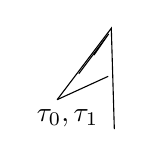
\begin{tikzpicture}[scale=.55]\draw (0,0)--(1.25,1.65)--(1.32,-.68);\draw (0,0)--(1.18,.54);\node[below] at (.24,0) {\deleted{$\unsure{\tau_0,\tau_1}$}};\draw (.5,.6)--(1.19,1.52)--(.85,1.03);\end{tikzpicture}}
\[
(V,\deleted{\unsure{f_0}}f_V,\{L_i\}_{0\leq i\leq n},a_0\}
\]

$V$ fibré vectoriel rang $n+1$

$f_V$ forme quadratique

$L_i$ sous-fibré vectoriel rg $1$\qquad $0\leq i\leq n$

$a_0$ \deleted{base} \inserted{section} de $L_0$ \deleted{(rigidification \ldots)}

a) $f_V|L_i$ lisse \deleted{[\unsure{et $\varphi|L_i$ est non dégénérée en tte fibre, en ce sens}]} $0\leq i\leq n$

b) $L_i\perp L_j$ si $0\leq i<j\leq n$ \quad $j,\deleted{\unsure{\leq|\ne}},i$ non consécutifs

c) $L_i\not\perp L_{i+1}$ sur \deleted{aucune} \inserted{tte} fibre $(0\leq i\leq n-1)$

d) $f(a_0)=1$ (normalisation pour $L_0$ et $f$ ]

Correspond aux \unsure{$n$-polyèdres|hyperpolyèdres} réguliers \unsure{pseud.|pseudo.} épinglés pour lesquels $\beta=\prod\beta_i$ inversible (mais $\widetilde\rho$ pas néc. inv, i.e. $f_V$ pas néc. lisse \ldots)

\diagram{\begin{tikzcd}[ampersand replacement=\&,column sep=.55em,row sep=1.7em]
\deleted{L_0}\arrow[dr,dash,"{\deleted{\tau_0}}"']\&\deleted{\unsure{L_1}}\arrow[d,dash]\&{}\&L_0\arrow[dl,dash,"{\tau_0}"']\arrow[dr,dash,"{\unsure{1|\tau_0}}"]\&{}\&L_1\arrow[dl,dash,"{\tau_1}"']\arrow[dr,dash]\&{}\\
{}\&\deleted{L'_0}\&L'_0\&{}\&L'_1\&{}\&L'_2
\end{tikzcd}\quad
\begin{tikzcd}[ampersand replacement=\&,column sep=.6em,row sep=1.7em]
{}\&L_i\arrow[dl,dash,"{\tau_i}"']\arrow[dr,dash,"{\unsure{1|\tau_i}}"]\&{}\&L_{i+1}\arrow[dl,dash]\\
L'_i\&{}\&L'_{i+1}\&{}
\end{tikzcd}\quad$\big|\,\beta_i$}

\[
L'_i=\psi_V(L_i)
\]

\[
\boxed{\varphi(a_i,a_{i+1})=-f(a_{i+1})}\ \text{\uline{inv.}}
\]
définit de proche en proche les \uline{bases} $a_i$ des $L_i$, à partir de $L_0$ déjà donnée

\[
a_i\in L_i\qquad\mathord{\tikz[baseline=(q.base)]{\node[inner sep=1pt] (q) {$a'_{i+1}=\psi(b_{i+1})$};\draw (q.center) ellipse (1.63cm and .38cm);}}
\]
\[
\langle a_i,a'_{i+1}\rangle=1\quad\text{i.e.}\quad \boxed{\varphi(a_i,b_{i+1})=1}
\]
\[
\deleted{a_{i+1}a'_{i+1}}\qquad
\mathrm{id}+\underbrace{a'_{i+1}}_{\deleted{\psi(b_{i+1})}}\otimes a_{i+1}=\tau_{i+1}
\]
\[
\left\{\begin{aligned}
a_{i+1}&=\unsure{\zeta_{i+1}|\gamma_{i+1}|\xi_{i+1}}b_{i+1}=\frac{-1}{f(b_{i+1})}b_{i+1}\\
\zeta_{i+1}&=-f(a_{i+1})\deleted{\unsure{\zeta_i|\xi_i|b_i}}=-\frac1{f(b_{i+1})}\\
&=-\zeta_{i+1}^2 f(b_{i+1})
\end{aligned}\right.
\]
\[
1=-\zeta_{i+1}f(b_{i+1})
\]
\[
\begin{aligned}
a'_{i+1}&=\frac{-1}{f(a_{i+1})}\psi(a_{i+1})\\
&=\psi\left[\underbrace{-\frac1{f(a_{i+1})}a_{i+1}}_{b_{i+1}}\right]\\
&\deleted{\unsure{\text{d'où }|b_{i+1}=}a_{i+1}=-\frac1{f(\unsure{a})}}
\end{aligned}
\]
\[
\varphi(a_i,a_{i+1})=\frac{1}{\deleted{\unsure{a_{i+1}}}}\zeta_{i+1}=-f(a_{i+1})
\]
\scanpage{34}
\[
\begin{aligned}
\varphi(a_i,a_{i+1})&=-\beta_0\cdots\beta_i\\
f(a_i)&=\deleted{\unsure{b|\beta}}\beta_0\cdots\beta_{i-1}&
\frac{\varphi(a_i,a_{i+1})^2}{f(a_i)\,f(a_{i+1})}&=\beta_i\,[=4\cos^2\theta_i]\\
f(a_{i+1})&=\beta_0\cdots\beta_i
\end{aligned}
\]
\[
\bigl[\alpha_i=\beta_i-2=2\bigl[\underbrace{2\cos^2\theta_i-1}_{\cos2\theta_i}\bigr]=2\cos2\theta_i\bigr]
\]
$\alpha_i$ est l'\uline{invariant de} $\tau_{a_i}\tau_{\unsure{a_{i+1}|i+1}}$ (rotation)

\figure{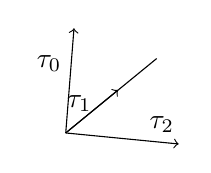
\begin{tikzpicture}[scale=.7]
\draw[->] (0,0)--(.15,1.9) node[left,pos=.66] {$\tau_0$};
\draw (0,0)--(1.65,1.35);
\draw[->] (0,0)--(.95,.78) node[left,pos=.68] {$\tau_1$};
\draw[->] (0,0)--(2.05,-.20) node[above,pos=.85] {$\tau_2$};
\end{tikzpicture}}
$\alpha_0,\alpha_1$
\[
\underbrace{\tau_0\ \tau_1}\ \tau_2\llap{$\underbrace{\phantom{\tau_1\ \tau_2}}$}
\qquad
\rho_0=\tau_0\tau_1\quad \rho_1=\tau_1\tau_2
\]
\figure{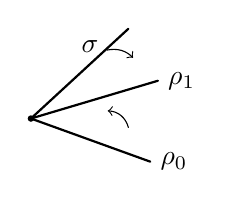
\begin{tikzpicture}[scale=.75,line cap=round]
\fill (0,0) circle (.055);
\draw[thick] (0,0)--(1.65,1.52) node[left,pos=.8] {$\sigma$};
\draw[thick] (0,0)--(2.15,.64) node[right] {$\rho_1$};
\draw[thick] (0,0)--(2.02,-.73) node[right] {$\rho_0$};
\draw[->] (1.29,1.16) to[bend left=27] (1.73,1.03);
\draw[->] (1.65,-.15) to[bend right=36] (1.30,.13);
\end{tikzpicture}}
\[
\tau_0=\rho_0\tau_1\qquad \tau_2=\tau_1\rho_1\qquad
\tau_0\tau_2=\rho_0\rho_1=\sigma\qquad \sigma^2=1\quad \text{i.e. }\tau_0,\tau_2\ \text{comm.}
\]
\[
\tau_0^2=\rho_0\tau_1\rho_0\tau_1=\rho_0\rho_0^{-1}=\mathrm{id}
\]

?? \uline{Prop} Soit
\[
\begin{aligned}
G_2&=(\underline{\tau}_0,\underline{\tau}_1,\underline{\tau}_2\mid
\underline{\tau}_0^2=\underline{\tau}_1^2=\underline{\tau}_2^2=(\underline{\tau}_0\underline{\tau}_2)^2=1)\\
\rotatebox{90}{$\hookrightarrow$}\quad &\\[-1ex]
G_2^+&=(\underline{\rho}_0,\underline{\rho}_1\mid(\underline{\rho}_0\underline{\rho}_{\unsure{+|1}})^2=1)
\end{aligned}
\]
\diagram{\begin{tikzcd}[ampersand replacement=\&,column sep=small]
\tau_0\tau_1 \& \tau_1\tau_2\\
\rho_0\arrow[u] \&\rho_1\arrow[u,dash]
\end{tikzcd}}

Considérons fibré projectif \inserted{$X$} sur $S$, \inserted{\deleted{\unsure{X}} de rg $N\geq1$} et \deleted{\unsure{catégorie|catégories}}, $G=\mathrm{Aut}(X)$. \deleted{Alors \illegible{1} Alors} Soit $\mathrm{Hom}^!(G_2,G)$ le sous-ensemble des $\mathrm{Hom}_{\mathrm{gr}}(G_2,G)$ formé des $\varphi$ telles que $\tau_i\overset{\mathrm{dfn}}{=}\varphi(\underline{\tau}_i)$ \unsure{soit|soient} une \uline{réflexion} $(i=0,1,2)$, et que $(\tau_0,\tau_1)\ (\tau_1,\tau_2)$ et $(\underbrace{\tau_0\tau_1}_{\unsure{\rho|{}}}\overset{\mathrm{dfn}}{=}\rho_0,\enspace \tau_1\tau_2\overset{\mathrm{dfn}}{=}\rho_{\unsure{2|1}})$ ne commutent pas \inserted{fibre par fibre} (i.e. $\rho_0^2\ne\mathrm{id}$, $\rho_1^{\unsure{2|{}}}\ne\mathrm{id}$, $\rho_0\rho_1\ne\rho_1\rho_0$ fibre \unsure{p|par} fibre.

% archive sheet number: 33
% slanted
\margin{\uline{NB} $\rho_0$ et $\rho_1$ ne \unsure{comm.} pas \unsure{entre eux} $\Longleftrightarrow$ $\tau_1$ et $\sigma$ ne commutent pas $\Longleftrightarrow$ $\sigma$ \unsure{fixe|permute} \unsure{autr.} les \illegible{1} \unsure{conditions|d'autres} \unsure{j'}\illegible{1} on \unsure{estime} que $\tau_0,\tau_2$ et $\sigma$ \unsure{ne soient permut.} pour cette \unsure{hypothèse}.}

Soit $\mathrm{Hom}^!(G_{\unsure{2|4}}^+,G)$ le sous-ensemble de $\mathrm{Hom}_{\mathrm{gr}}(G_2^+,G)$ formé des $\varphi^+$ telles que $[\deleted{\unsure{\rho=\varphi^+(\rho)}}\ \rho_0=\varphi^+(\underline{\rho}_0),\rho_1=\varphi^+(\underline{\rho}_1)]$ on ait : $\rho_0^2\ne1$, $\rho_1^{\unsure{2|{}}}\ne1$, $\rho_0\rho_1\ne\rho_1\rho_0$ sur chaque fibre, et (si $N\geq\deleted{\unsure{1}}2$) $\exists$ loc. sur \unsure{$S$|la base|{}} fibré projectif \inserted{de $Z$ de $X$, de codim $3$, et des} \deleted{tel que \unsure{fibre par fibre} $\rho_0|X_0=\rho_1|X_0=\mathrm{id}_{X_0}$.}
% long insertion from the foot of the sheet
\inserted{projectifs $X_0,X_1,X_2\supset Z$ de codim $2$, \inserted{$X_0\cap X_1\cap X_2=Z$,} tels que $\rho_0,\rho_1,\sigma=\rho_0\rho_1$ induisent l'identité resp. sur $X_0,X_1,X_2$ [si $N=2,3$ il faut \deleted{sans} doit \uline{se donner} les $X_i$, si $N\geq4$ ils sont uniques\ldots]}

\uline{Alors} l'application $\varphi\longmapsto\varphi^+=\varphi\mid G_2^+$ sera bijective. (?)

\margin{TSVP}
